\documentclass[11pt]{article}

\usepackage[utf8]{inputenc}
\usepackage{amsmath}
\usepackage{amssymb}
\usepackage{amsthm}
\usepackage{graphicx}
\usepackage{booktabs}
\usepackage[round]{natbib}
\usepackage[hidelinks]{hyperref}
\usepackage[margin=1in]{geometry}

\newtheorem{theorem}{Theorem}

% ============================================================
% TITLE
% ============================================================
\title{NeuralHorner: Learning a Modulus-Conditioned Transition for
Cross-Prime Modular Arithmetic under a Fixed Algorithmic Scaffold}

\author{Robert Sneiderman \\ Independent \\ \texttt{robbysneiderman@gmail.com}}

\date{}

\begin{document}
\maketitle

\begin{center}
\textit{Draft in progress, last updated 2026-08-11}
\end{center}

% ============================================================
% ABSTRACT
% ============================================================
\begin{abstract}
Computing $(a\,b)\bmod p$ across primes has a wall: monolithic learners reach
only limited success, circular regression and a sequence-to-sequence transformer
both fall short \citep{lauter2024modular}, and the sharper question is
cross-prime: whether one model can handle primes it never trained on. NeuralHorner clears that wall across all ten scored tiers of the challenge's
official scorer. The split of responsibility is stated plainly: a fixed,
hand-coded bit-serial Horner loop supplies the schedule, and a single learned cell
supplies the arithmetic. Learned modulus-conditioned Horner transitions and
cross-prime transfer precede this work \citep{xllent2026horner}; we claim a compact
single-cell implementation with learned operand reductions and the verification
and failure analysis below, not invention of the recurrence or discovery of the loop. The cell, a shared
$471$K-parameter bidirectional two-layer GRU, learns the per-step transition
$s' = (2s + d\,x)\bmod p$ and is re-run in that loop to reduce $a\bmod p$, reduce
$b\bmod p$, and multiply the residues. On the challenge's official open-source scorer, run by us
on a single H100 rented via RunPod, it scores exact-match $1.00$ on every one of tiers~$1$
through~$10$, for \texttt{overall\_accuracy} $1.00$ and
\texttt{highest\_tier\_above\_90} of~$10$ (the scorer's eleventh tier, tier~$0$, is a
pure-multiplication diagnostic excluded from the ranking metric, where the cell scores
$60/100$), reproduced identically across three
scorer-operand seeds of the single trained checkpoint (training initialization fixed). Each full run completes in $163$ to $174$ seconds, about
$125$ seconds inside the $300$-second budget, and the determinism re-run is
identical. The same shared cell handles every tier because inference sizes the
per-step state width to each prime's bit-length (dynamic-$L$). This is exact for
the symbolic recurrence; for the trained cell, the recorded $6/6$ comparison is
output-identical to full-width inference. Dynamic-$L$ brings the run under budget.

The model is not exact, and we say where. Randomizing the weights collapses every
tier of the weight-perturbation anti-cheat battery from $64/64$ to $0/64$, the
organizers' named anti-cheat condition, so the
capability sits in the trained parameters. The per-step transition is exact on
$40954$ transitions in total across all primes below $64$ (exhaustive). On first contact, a
structured battery whose families were disjoint from v8 training scored $759/768$
($98.83\%$); the only failures were Fermat numbers $2^{2^n}+1$. The battery later
became development data through DAgger and repair selection, so this is a historical
v8 diagnostic rather than a sealed post-selection estimate. It localizes a narrow
structural fragility at power-of-two-adjacent operands. A Lean~4
package machine-checks (axioms \texttt{propext} and \texttt{Quot.sound},
\texttt{sorry}/\texttt{admit}-free) the integer double-and-add-mod-$p$ algorithm
the loop imitates; it does not cover the learned network, and the cell-to-step
bridge is open. An immutable historical receipt for a conservatively interpolated
direct-two-pass/L2-SP candidate records all $193116$ selected exact-prefix
transition decisions as correct. Separate schedule-cost evidence shows that the
two-pass program lowers a source-bound recurrent bit-work proxy by $20.001\%$ on
the public scored-tier workload; this is an operation count, not measured latency.
The broader frozen-v3 retention run nevertheless failed: $509/512$ attempted
rows were exact, with errors at fixed-Hamming source indexes $003$, $035$, and
$110$; fail-closed stopping left the other $1024$ rows unrun. A crossed four-arm
ablation distinguishes a weight--schedule interaction, a schedule-caused error,
and a weight-caused error. Thus the local $F_{11}$ repair and the direct schedule
meet a measured Pareto wall rather than a global repair. The candidate was
neither submitted nor promoted and is stopped; submitted v8 remains the only
qualified artifact. The receipt-backed scorer result is self-run, while Rob's
separate automated-submission observation is unarchived; neither is a final
leaderboard ranking. No organizer compliance ruling is claimed: no question was
sent and no ruling was requested or issued.
\end{abstract}

% ============================================================
% INTRODUCTION
% ============================================================
\section{Introduction}
\label{sec:intro}

Learning $(a\,b)\bmod p$ across primes runs into a wall. A monolithic learner that
reads the whole operand pair and emits the whole product reaches only
limited success \citep{lauter2024modular}; the
same brittleness was recorded a decade earlier for bit-serial neural arithmetic
\citep{kaiser2016neural, price2016neural}. The SAIR Modular Arithmetic
Challenge\footnote{Official challenge repository: \url{https://github.com/SAIRcompetition/modular-arithmetic-challenge}.}
turns this into a graded test, scored by an open-source evaluation pipeline and
guarded by a weight-perturbation anti-cheat condition, and asks in its own framing
where a learned reducer breaks.

NeuralHorner clears all ten scored tiers. A single modulus-conditioned recurrent
cell, reused across a fixed bit-serial Horner loop, scores exact-match $1.00$ on
each of tiers~$1$ through~$10$ of the official scorer, for
\texttt{overall\_accuracy} $1.00$ and \texttt{highest\_tier\_above\_90} of~$10$,
reproduced identically across three seeds and within the time budget. Where the
monolithic framing reaches only limited success, the conditioned
cell transfers to unseen primes across the full tier ladder.

\paragraph{The construction.}
The method is one recurrent cell applied in a fixed Horner schedule. The cell, a
bidirectional two-layer GRU of about $471$K parameters, is conditioned on the
modulus $p$ and learns the per-step transition $s' = (2s + d\,x)\bmod p$, with the
data bit $d$ read from one operand and the control multiplier $x$ supplied by the
other. The same weights, re-run with different inputs, perform all three sub-tasks
the product needs: reduce $a \bmod p$ ($x{=}1$), reduce $b \bmod p$ ($x{=}1$), and
multiply the residues ($x = a\bmod p$, control bits from $b\bmod p$). State is
carried as bits throughout, per-argument preprocessing feeds one operand per hook,
and the loop schedule and bit packing are fixed by hand; only the cell is learned.

\begin{table}[t]
 \centering\small
 \begin{tabular}{lcl}
 \toprule
 Component & Learned? & Notes \\
 \midrule
 Bit order (MSB-first) & No & fixed schedule \\
 Number/order of passes & No & reduce $a$, reduce $b$, multiply \\
 Data bit $d$ vs.\ control $x$ & No & hand-assigned per pass \\
 State as a bit vector & No & fixed representation \\
 Per-step transition $s'$ & Yes & the shared GRU cell \\
 Dependence on the modulus $p$ & Yes & learned conditioning \\
 Output decoding & No & the official scorer \\
 \bottomrule
 \end{tabular}
 \caption{What is learned versus fixed. The algorithmic schedule is hand-coded; the
 per-step modular transition and its dependence on $p$ are learned. We claim this
 compact learned-reduction implementation and its measured boundary, not invention
 of modulus-conditioned Horner transfer or discovery of the schedule.}
 \label{tab:learned-vs-fixed}
\end{table}

\paragraph{One cell across every width, by dynamic sizing.}
A single weight set covers tiers whose primes span many bit-lengths because
inference sizes the per-step state width to each prime's bit-length (dynamic-$L$).
A canonical residue $s < p$ fits in $\lceil \log_2 p \rceil$ bits, so the bits a
narrower state would drop are always zero; reducing the width is therefore
exact for the symbolic recurrence; empirically, dynamic-$L$ and full-width inference
produce identical scorer outputs on every evaluated case: on a shared problem set,
fixed-$L$ (the full $2048$-wide state) and dynamic-$L$ both score $6/6$ with every
transition verified. This finite comparison does not prove equivalence for every
input of the bidirectional GRU. The scorer batches problems within a
tier, whose primes share a bit-length, so each batch sizes to a single width; any
modest within-tier spread is handled by sizing to the batch maximum. On the
recorded comparison, batch masking changed no answer. This sizing also removes the wasted
compute that a fixed maximum width spends on the easy tiers, and it is the reason a
full ten-tier run finishes in $163$ to $174$ seconds, roughly $125$ seconds under
the $300$-second budget. The per-step cost scales with the state width $L$ (the GRU runs over $L$ positions
each step), so CUDA graph capture, which only removes launch overhead, was slower
than the eager baseline ($402$\,s versus $383$\,s); the gain came from narrowing the
per-step state ($383$\,s to $163$--$174$\,s).

\paragraph{Where exactness holds and where it fails.}
The forward path carries no shortcut. It contains no symbolic-math call, no
big-integer modular multiply, no lookup table, and no comparison against $p$ in
Python or in tensor operations; randomizing the cell's weights collapses every
tier from $64/64$ to $0/64$ exact-match, the organizers' own named anti-cheat
condition. Per step, the learned transition matches $(2s + d\,x)\bmod p$ on
$40954$ transitions in total (every $s,x,d$ triple) across all primes below $64$, checked exhaustively.
The full chain is another matter. On first contact, a structured battery whose
families were disjoint from original v8 training scored $759/768$ ($98.83\%$):
Fibonacci-valued operands,
alternating bits, fixed-Hamming-weight operands, quotient-correlated operands,
and primes $p \equiv 3 \pmod 4$ were each perfect at $128/128$, and the only
failures were Fermat numbers $2^{2^n}+1$ ($119/128$). All $9$ misses were
power-of-two-adjacent. Later repair selection used these cases, so the battery is
now frozen development data rather than a sealed estimate for new candidates. A
separate Lean~4 development machine-checks, free of \texttt{sorry}
and \texttt{admit} and under axioms \texttt{propext} and \texttt{Quot.sound}, that
the integer double-and-add recurrence the loop imitates equals $(a\,b)\bmod p$ for
any bit length with the canonical-residue bound. It also proves a conditional
exact-prefix bridge: agreement of an arbitrary transition cell with the exact
step at every exact trajectory state implies equality of the complete scan, and
two such certificates compose for the direct two-pass product. The hypotheses
remain empirical for NeuralHorner; ``provably exact'' attaches only to the
algorithm and the stated conditional bridge.

\paragraph{Contributions.}
\begin{enumerate}
\item \textbf{A compact shared cell with learned operand reductions.} One shared
modulus-conditioned cell, reused across a fixed bit-serial Horner schedule, transfers
the learned per-step reduction across unseen primes, clearing every one of tiers~$1$
through~$10$ at exact-match $1.00$ on the official open-source scorer (self-run on a rented RunPod H100,
three scorer-operand seeds, within budget; \texttt{overall\_accuracy} $1.00$, highest
cleared tier~$10$), where monolithic learning of the task reaches only limited success
\citep{lauter2024modular}. The comparison is not like-for-like: a monolithic learner
fits the whole operand-to-product map, whereas this cell learns only the per-step
transition inside a fixed scaffold. XllentAI previously reported the same learned
modulus-conditioned Horner formulation and held-out-prime transfer
\citep{xllent2026horner}. NeuralHorner's distinction is one roughly $471$K-parameter
BiGRU checkpoint across the full tier ladder, with both operand reductions also
performed by the learned cell rather than Python-side \texttt{\% p}. This is an
implementation and empirical result, not a claim to the shared formulation.
\item \textbf{A precise exactness boundary, with a machine-checked algorithm.} Per-step
receipts (exhaustive over $40954$ transitions in total across all primes below $64$), a
weight-perturbation provenance check ($64/64 \to 0/64$), a $\mathrm{bf16}$ decision
check that matches $\mathrm{fp32}$ on its recorded battery, and a first-contact structured battery
($759/768$) that localized every submitted-v8 failure to the
power-of-two-adjacent (Fermat) family before becoming development data,
refining the symmetric-input brittleness \citet{price2016neural} report for the Neural
GPU. A separate Lean~4 proof machine-checks that the integer double-and-add recurrence
equals $(a\,b)\bmod p$ for any bit length with the canonical-residue bound
(\texttt{sorry}/\texttt{admit}-free; axioms \texttt{propext}, \texttt{Quot.sound}).
It also formalizes why exact-prefix transition certificates imply a complete
scan and why certified reduction and direct-scan passes compose. It does not
prove that the trained checkpoint satisfies those hypotheses beyond a tested
trajectory, and network exactness is never claimed.
\item \textbf{Dynamic-$L$ inference and a per-step-compute speed finding.} Sizing the
per-step state width to each prime's bit-length is exact for the symbolic recurrence and
empirically output-identical to full-width inference on the recorded $6/6$
comparison, and brings a ten-tier run to $163$--$174$\,s, about $125$\,s under
budget. The workload is depth-bound, so CUDA graphs lost to the eager baseline and the
speedup came from narrowing the state rather than from kernel fusion.
\item \textbf{A failed repair resolved causally rather than hidden.} A canonical
direct two-pass program plus an L2-SP interpolation is recorded by the immutable
historical receipt as clearing a selected frozen-v3 $F_{11}$ exact-prefix gate,
but a broader receipt-bound run fails at three
fixed-Hamming cases. Crossing original/direct schedules with v8/repaired weights
separates schedule, weight, and interaction failures. This negative result
rejects promotion and shows that local counterexample repair can relocate error
even when its target family is closed; it is evidence about the present frontier,
not evidence that no global repair exists.
\end{enumerate}
The compact implementation, boundary, and verification results hold regardless of the organizer's
ruling on the fixed schedule.

\paragraph{Scope of the claims.}
This work is not a verified learned multiplier: the proof covers the integer
algorithm, and the cell-to-step bridge is open. The model is not exact: the
power-of-two-adjacent residual is real in the submitted-v8 first-contact result,
but the battery is no longer sealed evidence after repair selection. The score is the official scorer run by us; it is not
organizer-leaderboard-verified at scale, the timing was measured on a rented RunPod H100 and
the organizers' hardware may differ, and the compliance status of the hand-fixed
Horner schedule has not yet been ruled on; a clarification question is drafted but
has not been sent.

% ============================================================
% RELATED WORK
% ============================================================
\section{Related Work}
\label{sec:related}

The pieces this method uses are established. It recombines bit-serial neural
arithmetic, weight sharing in a fixed loop, and a finite-state reading of the
recurrence; it is not a new architecture. The paragraphs below place each component
beside its source and state where this work differs, with novelty deliberately
underclaimed.

\paragraph{Neural arithmetic and its fragility.}
The Neural GPU \citep{kaiser2016neural} showed that a recurrent convolutional cell
can learn bit-serial binary arithmetic and extend to input lengths well beyond
those seen in training. \citet{price2016neural} then characterized its failure
mode: a Neural GPU trained to apparent exactness on random operands still errs on
structured inputs, and families such as powers of two times a random residue
expose carries the model never learned. The submitted v8 checkpoint reproduces
both halves of that finding and sharpens the second. It matches the
random-operand scorer exactly on every tier, and a first-contact structured
battery surfaces a residual; that residual is
not diffuse, it is confined to the power-of-two-adjacent Fermat family
(Section~\ref{sec:results:battery}). The reading we take from
\citet{price2016neural} is that passing a random-operand scorer is not exactness,
and we report the result on those terms.

\paragraph{Compiling exact programs into networks.}
RASP \citep{weiss2021rasp} is a small language whose primitives map onto attention
and feed-forward operations, and Tracr \citep{lindner2023tracr} compiles RASP
programs into concrete transformer weights, yielding networks that are exact by
construction. That line answers a different question. There the symbolic program is
known in advance and installed into the weights; here the per-step transition is
learned from operand-output pairs, and exactness is an empirical property to be
measured rather than a guarantee inherited from a compiler. The two lines meet only
at the formal artifact of Section~\ref{sec:lean}, which machine-checks the integer
algorithm and says nothing about the learned cell.

\paragraph{Looped and weight-shared computation.}
Applying one shared cell in a fixed loop, with depth set by input length rather
than by a learned halting rule, places this work next to looped transformers
\citep{fan2024looped}, which reuse a single block across iterations to extend the
reachable computation and improve length generalization on tasks expressible as
iterated steps. The shared modulus-conditioned cell here plays the same structural
role inside a Horner schedule. A single modulus value steers the cell across many
primes. That mechanism is shared with the Horner-RNN described below; the result
here concerns its compact single-checkpoint realization with learned operand
reductions.

\paragraph{Neural algorithmic reasoning.}
Training a network to align with a classical algorithm, rather than to discover it
end to end, is the premise of neural algorithmic reasoning \citep{velickovic2021nar}; the
idea of a learned executor separate from program structure goes back to neural
programmer-interpreters \citep{reed2016npi}, and \citet{bohde2024markov} argue that
algorithmic steps are Markovian, so a learned transition over the current state
generalizes better than one carrying history, which is what the per-step cell here
does. Relatedly, transformers length-generalize on a task when it admits a short
program in a transformer-expressible language \citep{zhou2023rasp}. Fixing the Horner schedule
and learning only the per-step transition is one extreme of that trade-off, maximal
algorithmic alignment, and it raises the question of how much of the schedule can be
handed back to the network before transfer breaks.

\paragraph{The monolithic modular-multiplication wall.}
\citet{lauter2024modular} study modular multiplication with circular regression and
a sequence-to-sequence transformer and report only limited success, which
they read as evidence of the task's hardness; the same crypto-ML line trains
transformers on modular arithmetic inside lattice attacks \citep{salsa2022}, but for
probabilistic secret recovery rather than exact arithmetic, so exact cross-prime
extrapolation is a different bar. The
monolithic reference baselines shipped with the challenge agree, clearing only the
easiest tier. For the easier operation of modular \emph{addition},
\citet{mccracken2025modadd} find that multilayer perceptrons and transformers
converge on a common abstract algorithm, an approximate Chinese Remainder Theorem;
multiplication is harder, and we supply the schedule rather than learn it. The
observation here is that the wall tracks the monolithic, cross-prime, large-modulus framing rather than
learned modular multiplication as such. Conditioning a single bit-serial cell
on the modulus, and reducing each operand and multiplying residues with the same
shared weights, transfers across unseen primes through every tier.

\paragraph{Nearest learned-Horner prior art.}
The XllentAI \texttt{modular\_arithmetic} repository predates NeuralHorner's
GitHub release and supplies the nearest formulation \citep{xllent2026horner}: a
hard binary recurrent state, a learned modulus-conditioned
Horner/double-and-add transition, and reported transfer to held-out primes. Its
historical June~13 revision routes among three width-specific MLP cells and
reports public performance through $64$-bit primes. Its June~22 revision reports
two shared carry-aware TCN weight sets (about $10.7$M parameters total), public
exact-match $1.00$ on tiers~$1$--$10$, true-trajectory state training,
width-distribution matching, worst-bit margin objectives, distillation, and
weight soups. We have not independently rerun those author-reported results. In
both pinned inference revisions, Python computes \texttt{a \% p} and
\texttt{b \% p} before the learned scan. NeuralHorner instead uses one roughly
$471$K-parameter BiGRU checkpoint for all challenge widths and runs the learned
cell to reduce both operands before multiplication. These are implementation,
efficiency, and evaluation distinctions; the shared Horner formulation and
cross-prime-transfer idea are not contributions of this work. Compliance of any
fixed schedule or operand normalization remains an organizer decision.

\paragraph{Grokking and mechanistic interpretability.}
A parallel line shows monolithic networks can learn modular arithmetic \emph{exactly},
but on a single fixed, small modulus. Networks grok modular tasks long after overfitting
\citep{power2022grokking}; the learned circuit has been reverse-engineered as a
discrete-Fourier ``clock'' for modular \emph{addition} \citep{nanda2023progress}, and
analytic weight solutions are known \citep{gromov2023grokking}. Two gaps separate that
setting from ours: the modulus is fixed and tiny, with no cross-prime transfer and no
cryptographic bit-lengths, and the clean Fourier structure is specific to addition.
Multiplication does not grok as cleanly, a $100$k-step probe with weight decay (the
canonical grokking setup) on the multiplication task produced no generalization jump,
consistent with \citet{mccracken2025modadd} placing multiplication beyond the
approximate-CRT addition circuit. The wall is therefore specific to cross-prime,
large-modulus multiplication, not to learned modular arithmetic in general.

\paragraph{Automata and finite-state readings of recurrent nets.}
A long line treats recurrent networks as finite-state machines; deterministic
automata can be extracted from trained RNNs \citep{weiss2018automata}. The
bit-serial Horner loop used here is a finite-state transducer over the bits of one
operand, with the learned cell as its transition function and the modulus as a side
input. On that reading the method is an instance of this program, not a departure
from it.

\paragraph{Position of this work.}
None of the above is claimed as a new mechanism. Bit-serial neural arithmetic,
weight sharing in a loop, modulus-conditioned learned Horner transitions, their
cross-prime transfer, and the transducer reading are all prior art. The position
of this work is narrower: one approximately $471$K-parameter BiGRU checkpoint
performs learned reductions and multiplication across the full tier ladder; its
dynamic-width cost, exactness boundary, and causal/provenance checks are reported
with receipts. The clean random-operand pass together with a narrow
power-of-two-adjacent fragility refines the residual of
\citet{price2016neural}. We claim the compact implementation, learned-reduction
path, and characterization, not the shared formulation or architecture.

% ============================================================
% METHOD
% ============================================================
\section{Method}
\label{sec:method}

\begin{figure}[t]
\centering
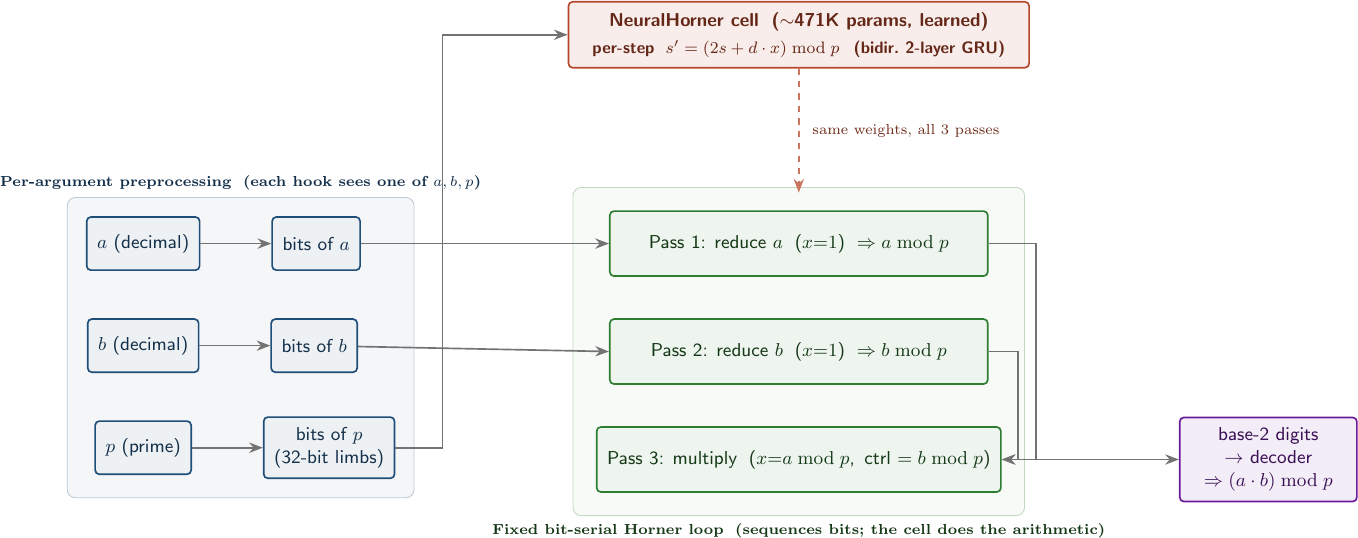
\includegraphics[width=0.66\linewidth]{figs/architecture.png}
\caption{NeuralHorner. One shared, modulus-conditioned cell learns the per-step
transition $s'=(2s+d\,x)\bmod p$ and is re-run with different inputs across a fixed
bit-serial Horner loop to reduce $a$, reduce $b$, and multiply the residues. The
loop schedule and bit packing are fixed; only the cell is learned, and randomizing
its weights collapses every tier to $0$.}
\label{fig:architecture}
\end{figure}

\subsection{Per-step transition}
\label{sec:method:step}

The method rests on one recurrent transition over residues modulo a prime $p$.
Write the state $s \in \{0,1,\dots,p-1\}$ as a canonical residue, take a control
multiplier $x$, and read a single binary data bit $d \in \{0,1\}$. The transition
is
\begin{equation}
 s' \;=\; (2s + d\,x) \bmod p .
 \label{eq:step}
\end{equation}
Starting from $s=0$ and iterating \eqref{eq:step} most-significant-bit (MSB) first
over the bits of an integer $m$ computes $(x \cdot m) \bmod p$, the left-to-right
double-and-add form of modular multiplication. Setting $x=1$ turns the same
recurrence into a reduction: $s' = (2s + d) \bmod p$ accumulates the bits of $m$
into $m \bmod p$. Bit-serial recurrences of this shape have a long lineage in
learned arithmetic \citep{kaiser2016neural}; the recurrence itself is the classical
double-and-add schedule and is not new here.

\subsection{Shared \texorpdfstring{$p$}{p}-conditioned cell}
\label{sec:method:cell}

A single recurrent cell realizes \eqref{eq:step}. The cell is a bidirectional
two-layer gated recurrent unit (GRU) of roughly $471$K parameters, conditioned on
the modulus $p$: at each step the cell reads the current state as a bit vector, the
data bit $d$, the control multiplier $x$, and a conditioning input derived from
$p$, and it writes the next state as a bit vector. The state is carried as bits
throughout, never as a wide integer. One weight set serves every step of every
phase below; no parameter is specialized to a particular prime, and the modulus
enters only through the conditioning input. The submission entry class is
\texttt{model.BitSerialReducer}, which wraps this cell with the fixed loop and the
preprocessing described next.

\subsection{Bit-serial Horner loop and the reduce/reduce/multiply composition}
\label{sec:method:horner}

A modular product $(a \cdot b) \bmod p$ is produced by three passes of the same
cell over a fixed bit-serial Horner schedule, with no learned control flow between
passes.

\paragraph{Reduce $a$.} Run \eqref{eq:step} with $x=1$ and the data bits set to the
bits of $a$, MSB first, giving $a \bmod p$.

\paragraph{Reduce $b$.} Run the same cell with $x=1$ and data bits set to the bits
of $b$, giving $b \bmod p$.

\paragraph{Multiply.} Run the cell with control multiplier $x = a \bmod p$ and data
bits set to the bits of $b \bmod p$, MSB first, giving
$\big((a \bmod p)(b \bmod p)\big) \bmod p = (a \cdot b) \bmod p$.

The schedule is fixed by hand and identical across primes: the number of steps, the
bit order, and which argument supplies $x$ versus the data stream are not learned.
Only the cell weights are learned, and the three phases reuse them without
modification. Per-argument preprocessing feeds one input per hook, so each hook
sees exactly one of $a$, $b$, $p$ rather than the full triple, which is what lets a
single conditioning value steer the cell across primes.

\subsection{Dynamic state-width inference}
\label{sec:method:dynl}

One weight set covers every scored tier, whose primes range over many bit-lengths,
because inference sizes the per-step state width $L$ to the bit-length of the prime
at hand rather than to a fixed maximum. A canonical residue satisfies $s < p$ and
so fits in $L = \lceil \log_2 p \rceil$ bits; any wider representation pads the
high bits with zeros. Narrowing the carried state to $L$ is therefore exact for the
symbolic recurrence. For the trained bidirectional GRU, full-width and dynamic-$L$
inference were output-identical on the recorded $6/6$ comparison with every
transition verified; this finite check is not a theorem for all inputs. Dynamic-$L$
is distinct from
training a separate model per width: the same trained cell is run at each tier with
its state sized to that tier's primes. Bit extraction uses $32$-bit limbs so that a
modulus $p \ge 2^{63}$ never overflows an integer tensor at the larger widths.

\subsection{Why CUDA graphs lost: the cost is per-step compute}
\label{sec:method:speed}

The dominant cost of a run is the per-step computation: each outer Horner step runs
the GRU over the full $L$-position state, so the total work scales with the state
width $L$. Two observations follow, both measured. First, capturing the loop as a
CUDA graph, which removes CPU launch overhead, made the run \emph{slower}, $402$
seconds against a $383$-second eager baseline: when the bottleneck is the per-step
compute rather than launch dispatch, graphs save little and their capture and
input-staging add overhead. Second, the effective lever is the per-step compute
itself, which dynamic state-width sizing (Section~\ref{sec:method:dynl}) reduces by
not carrying maximum-width state on the easy tiers, where the extra positions are
zero; this took the run from $383$ seconds to $163$--$174$ seconds. The speed result
is therefore that narrowing the per-step state, not amortizing launches, is what
brings a ten-tier evaluation comfortably under the $300$-second budget.

\subsection{Output, scorer decoding, and provenance}
\label{sec:method:output}

The final state is emitted in base $2$ as a bit string. The official open-source
scorer decodes this string to an integer and tests it for exact match against the
reference value $(a \cdot b) \bmod p$. The forward path performs no comparison
against $p$, no big-integer modular multiply, no lookup, and no symbolic
arithmetic, in either Python or tensor operations; the canonical-residue range is
produced by the recurrence, not by a clamp applied after the fact. The path is
checked under the organizers' weight-perturbation protocol: replacing the cell
weights with random values of the same shape collapses every solved tier from
$64/64$ to $0/64$ exact-match. A lookup table, a big-integer modular multiply, or
any direct-arithmetic routine would still answer correctly under random weights,
because its output does not depend on the trained parameters; only a model whose
answer is carried by the learned cell collapses to the floor when those weights are
randomized. Combined with the absence of any modular-arithmetic primitive in the
forward path, the collapse indicates that the solved tiers are produced by the
learned recurrence and not by a hidden symbolic shortcut.

% ============================================================
% RESULTS
% ============================================================
\section{Results}
\label{sec:results}

The challenge poses a wall and asks where it breaks. This section reports that the
wall falls across the whole tier ladder, then states precisely where the model is
still not exact. All numbers are from the challenge's official open-source scorer,
run on a single H100 rented via RunPod. Scoring follows the official rule:
\texttt{overall\_accuracy} is the equal-weight mean of per-tier exact-match over
tiers~$1$--$10$, and \texttt{highest\_tier\_above\_90} is the largest tier index at
or above $90\%$.

\subsection{All ten tiers at exact-match 1.00}
\label{sec:results:tiers}

Every scored tier returns exact-match $1.00$ (Table~\ref{tab:tiers},
Figure~\ref{fig:tier-progression}). The resulting \texttt{overall\_accuracy} over
tiers~$1$--$10$ is $1.00$ and \texttt{highest\_tier\_above\_90} is $10$. The separate
weight-perturbation anti-cheat battery scores each tier at $64$ cases: under the
trained weights every tier is $64/64$, and under randomized weights every tier drops
to $0/64$. The three monolithic
reference learners shipped with the challenge clear only the easiest tier, matching
the limited success of monolithic learners reported by \citet{lauter2024modular}; the
modulus-conditioned cell transfers to unseen primes across all ten.

Outside the scored tiers, the scorer's Tier-0 diagnostic isolates multiplication from
modular reduction; the cell scores $60/100$ there, failing on large operands. The learned
computation realizes $(a\,b)\bmod p$ inside its reduce-reduce-multiply training regime,
not as a general large-integer multiplier. We therefore scope the claim to modular
multiplication on the scored distribution, not pure multiplication, the same
distribution-specific brittleness as the power-of-two-adjacent residual.

\begin{table}[t]
 \centering
 \small
 \begin{tabular}{cccccc}
 \toprule
 Tier & Seed \texttt{a1a1a1a1} & Seed \texttt{b2b2b2b2} & Seed \texttt{c3c3c3c3}
 & Pooled & Randomized weights \\
 \midrule
 1 & 64/64 & 64/64 & 64/64 & 192/192 & 0/64 \\
 2 & 64/64 & 64/64 & 64/64 & 192/192 & 0/64 \\
 3 & 64/64 & 64/64 & 64/64 & 192/192 & 0/64 \\
 4 & 64/64 & 64/64 & 64/64 & 192/192 & 0/64 \\
 5 & 64/64 & 64/64 & 64/64 & 192/192 & 0/64 \\
 6 & 64/64 & 64/64 & 64/64 & 192/192 & 0/64 \\
 7 & 64/64 & 64/64 & 64/64 & 192/192 & 0/64 \\
 8 & 64/64 & 64/64 & 64/64 & 192/192 & 0/64 \\
 9 & 64/64 & 64/64 & 64/64 & 192/192 & 0/64 \\
 10 & 64/64 & 64/64 & 64/64 & 192/192 & 0/64 \\
 \midrule
 \multicolumn{4}{l}{\texttt{overall\_accuracy}} & $1.00$ & $0.00$ \\
 \multicolumn{4}{l}{\texttt{highest\_tier\_above\_90}} & $10$ & $0$ \\
 \bottomrule
 \end{tabular}
 \caption{Per-tier exact-match on the weight-perturbation anti-cheat battery (single
 rented H100): $64$ cases per tier per seed, for each of the three seeds and pooled
 across them. Every tier is $64/64$ under the trained weights and $0/64$ under
 randomized weights, and the corresponding \texttt{overall\_accuracy} /
 \texttt{highest\_tier\_above\_90} collapse from $1.00/10$ to $0.00/0$. Pooling the
 three seeds gives $192/192$ per tier, a $95\%$ Clopper--Pearson interval of
 $[0.981, 1.000]$ on the per-tier exact-match rate. The official scorer ($100$
 problems per scored tier) is reported in the text, not this table.}
 \label{tab:tiers}
\end{table}

\begin{figure}[t]
 \centering
 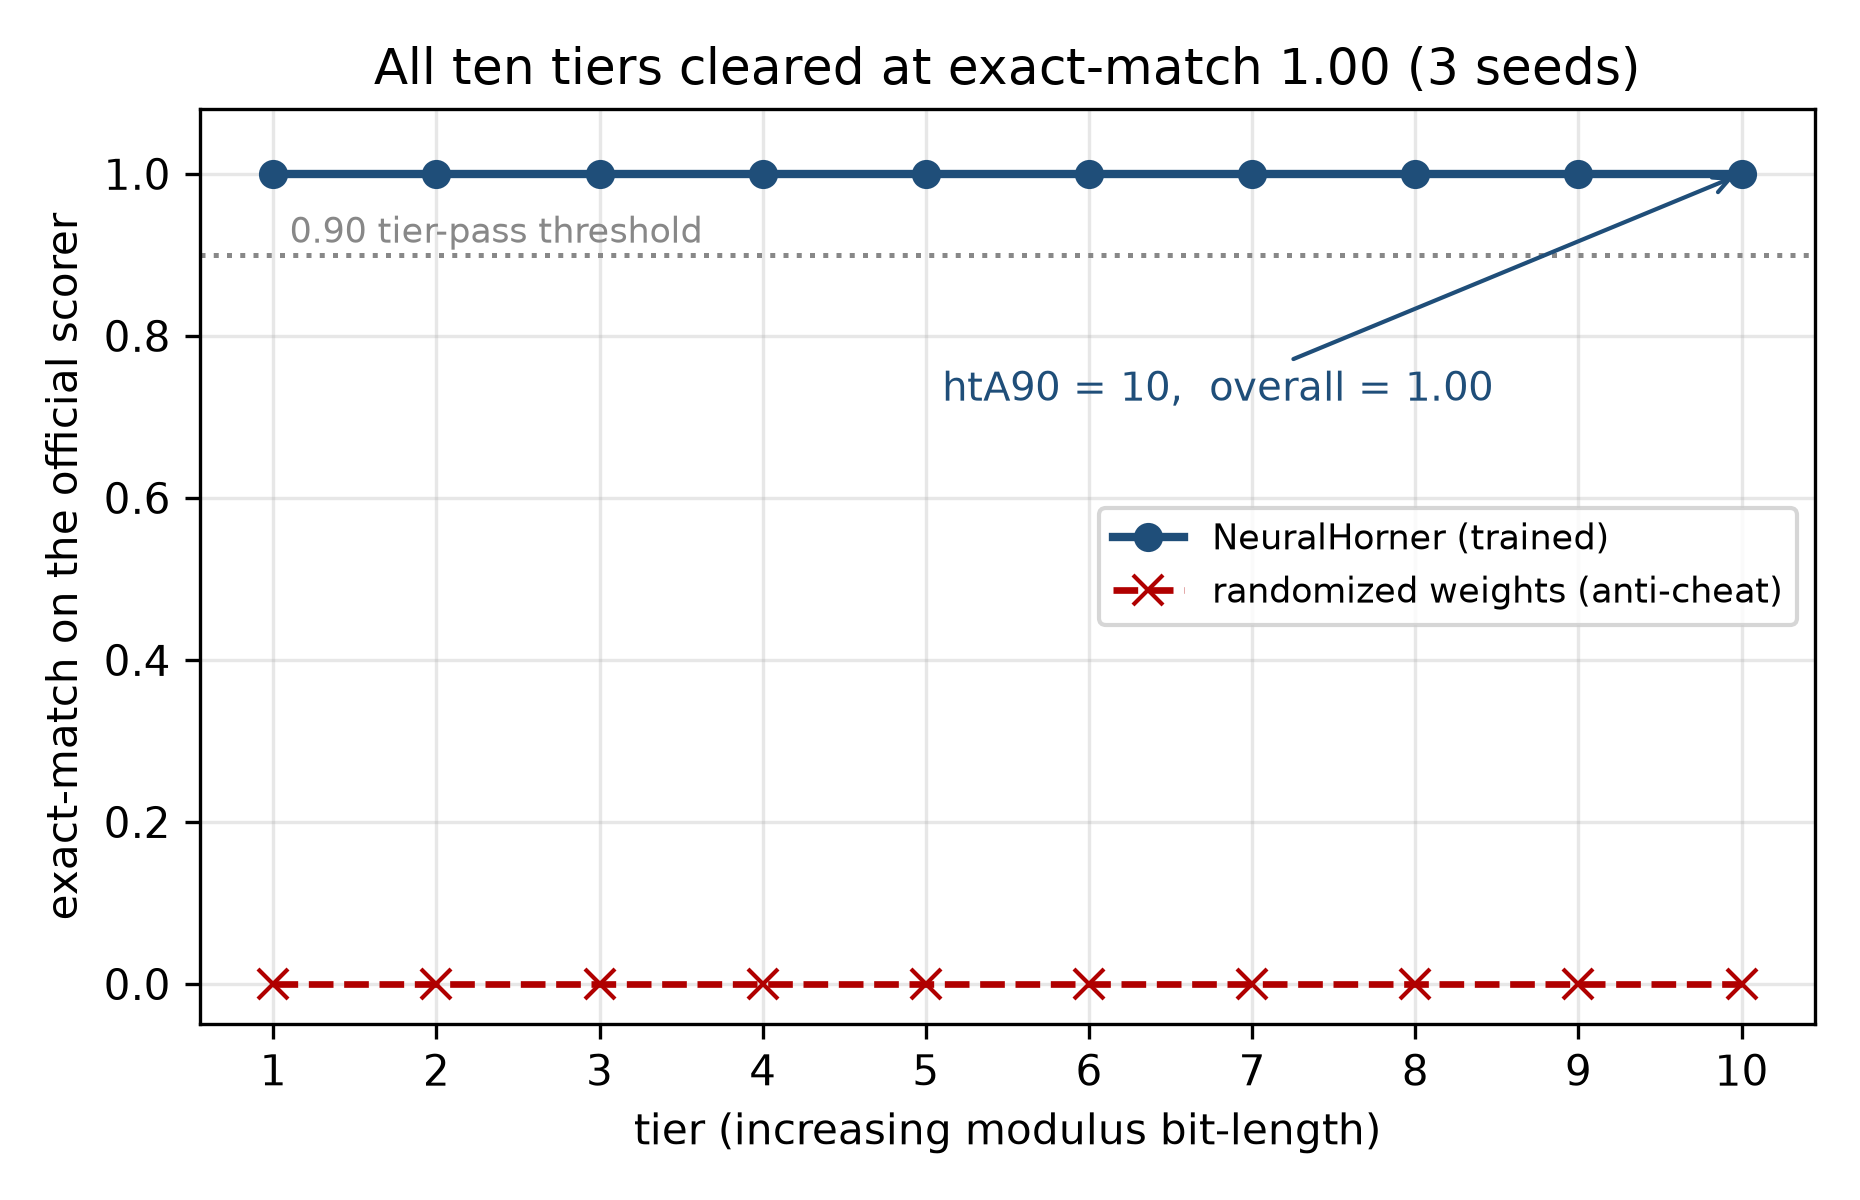
\includegraphics[width=0.78\linewidth]{figs/tier_progression.png}
 \caption{Exact-match on the official scorer for every scored tier. The trained
 cell scores $1.00$ on all ten tiers (\texttt{highest\_tier\_above\_90}~$=10$,
 \texttt{overall\_accuracy}~$=1.00$), reproduced across three seeds; randomizing
 the weights collapses every tier to $0$, the organizers' anti-cheat condition.}
 \label{fig:tier-progression}
\end{figure}

\subsection{Three seeds, timing, and determinism}
\label{sec:results:seeds}

The result holds across seeds and inside the time budget (Table~\ref{tab:seeds}).
Three runs that reseed only the scorer's random operand draws on the single trained
checkpoint (\texttt{a1a1a1a1}, \texttt{b2b2b2b2}, \texttt{c3c3c3c3}) each return \texttt{overall\_accuracy} $1.00$ and
\texttt{highest\_tier\_above\_90} $10$. A full ten-tier run completes in $163$ to
$174$ seconds on the rented H100, about $125$ seconds under the $300$-second budget, and
re-running a fixed seed reproduces both the answers and the score exactly.

\begin{table}[t]
 \centering
 \small
 \begin{tabular}{lccc}
 \toprule
 Seed & \texttt{overall\_accuracy} & \texttt{highest\_tier\_above\_90} & Wall-clock (s) \\
 \midrule
 \texttt{a1a1a1a1} & $1.00$ & $10$ & $163$--$174$ \\
 \texttt{b2b2b2b2} & $1.00$ & $10$ & $163$--$174$ \\
 \texttt{c3c3c3c3} & $1.00$ & $10$ & $163$--$174$ \\
 \bottomrule
 \end{tabular}
 \caption{Three scorer-operand seeds of the single trained checkpoint on the official scorer (single rented H100). Each run
 clears all ten tiers within the $300$-second budget; wall-clock spans $163$ to
 $174$ seconds across the three. The determinism re-run is identical.}
 \label{tab:seeds}
\end{table}

\subsection{Precision: bf16 decisions match fp32}
\label{sec:results:bf16}

On the recorded backend and frozen structured battery, $\mathrm{bf16}$ flips $0$
answers relative to $\mathrm{fp32}$, and the smallest observed decision margin is
$\min |\text{logit}| = 3.017$. This is battery-scoped agreement, not evidence that
all scorer results or other backends are floating-path invariant. The primary
output log is absent from this workspace, so this is labeled
\texttt{LOCAL-RESULT/UNARCHIVED}; the checking script remains available.

\subsection{Per-step exactness and provenance}
\label{sec:results:perstep}

The learned transition was checked directly against $(2s + d\,x)\bmod p$.
Exhaustively, over every state $s \in [0,p)$, every multiplier $x \in [0,p)$, and
both control bits $d \in \{0,1\}$, for every prime $p < 64$, all $40954$
transitions matched ($40954/40954$). This certifies the single-step map on this finite small-prime domain; it does
not by itself certify the full Horner chain at large prime sizes, where the
composition of many soft steps is exactly what the frozen structured battery below probes.
The weight-perturbation provenance check
(Section~\ref{sec:method:output}) supports that the answers are carried by the learned cell: every solved tier collapses from
$64/64$ to $0/64$ when the trained weights are replaced by random values of the
same shape, so the answers are carried by the learned cell rather than by a hidden
solver. This is the organizers' anti-cheat condition; on its own it shows only that
the fixed schedule does not compute the answer and the trained weights do, which is
the property that separates the entry from a hand-coded circuit.

\paragraph{Ablations.}
Two interventions on a shared problem set isolate what carries the computation.
Fixed-$L$ inference (the full $2048$-wide state) and dynamic-$L$ both score $6/6$ with
every transition verified, so dynamic-$L$ is output-equivalent on the evaluated cases.
Zeroing the modulus conditioning drops accuracy to $0/6$, so the dependence on $p$ is
load-bearing rather than incidental; randomizing the cell's weights collapses every
tier to $0/64$, so the trained weights, not the fixed loop, produce the answer.

\paragraph{Layered verification.}
We organize the exactness evidence in three complementary levels. Level~1
is the Lean proof of the integer recurrence (Section~\ref{sec:lean}). Level~2 is the
exhaustive single-step check above, $40954/40954$ on the small-prime domain. Level~3
is \emph{per-step trace verification}: along an evaluated rollout we log every triple
$(s,x,d)$ the cell consumes and check the emitted $s'$ against $(2s + d\,x)\bmod p$,
so a passing rollout carries a step-by-step record rather than only a matching
final answer, and a failing rollout is localized to its first divergent step. The harness verifies
every transition on random-operand rollouts at every depth checked: $1440/1440$ on
small primes, and $3088/3088$, $9228/9228$, and $12294/12294$ on tiers~$8$, $9$,
and~$10$ ($256$-, $1024$-, and $2048$-bit primes). On the failing Fermat inputs it
localizes the first divergent step (Section~\ref{sec:results:battery}). The levels are honest about
scope: this per-step check covers the evaluated rollouts, not all inputs, and the
cell-to-step bridge to a global proof of the network remains open.

\subsection{The fragility is narrow: power-of-two-adjacent operands}
\label{sec:results:battery}

A $1.00$ scorer pass on random operands is not exactness. A structured battery
whose six families were disjoint from the original v8 training data was first
scored only after that checkpoint was frozen. On this first-contact evaluation,
$128$ cases per family were scored at the top band (Table~\ref{tab:battery},
Figure~\ref{fig:exactness}). The cell is exact
on five of the six families, $128/128$ each: Fibonacci-valued operands,
alternating-bit operands, fixed-Hamming-weight operands, quotient-correlated
operands, and primes $p \equiv 3 \pmod 4$. The
single exception is Fermat numbers $2^{2^n}+1$, at $119/128$. All $9$ failures in
the battery are Fermat cases. Overall the battery is $759/768 = 98.83\%$ by row.
These are fixed-suite row counts, not $768$ independent draws: there are $693$
unique numerical $(a,b,p)$ cases, and the alternating-pattern family contains
only $53$ unique cases among its $128$ rows.

The official scorer runs $100$ problems per tier across $11$ tiers ($0$--$10$,
$1100$ problems in total), distinct from the separate $64$-case-per-tier
weight-perturbation battery used for the anti-cheat check (Table~\ref{tab:tiers}).
The ranking metrics \texttt{overall\_accuracy} and \texttt{highest\_tier\_above\_90}
are computed over the ten scored tiers $1$--$10$ ($1000$ problems); tier~$0$ is
excluded from them. On the scorer counts, exact (Clopper--Pearson) $95\%$ confidence
intervals are: each scored tier ($100/100$) is $[0.964, 1.000]$, the ten-tier scored
battery ($1000/1000$, tiers $1$--$10$) is $[0.9963, 1.000]$. We do not attach a
binomial sampling interval to the deliberately constructed, partially duplicated
structured battery. Tier~$0$ scores $60/100$ and does not enter the ranking metric; it
is the scorer's pure-multiplication diagnostic (Section~\ref{sec:results:tiers}), which
the cell does not fully clear because it realizes $(a\,b)\bmod p$ within its
reduce-reduce-multiply regime, not as a general large-integer multiplier. The failures are not spread across the Fermat
family either: they concentrate at the largest tested power-of-two-plus-one operand,
$F_{11} = 2^{2048}+1$ (a $2049$-bit operand at the top of the trained width range),
paired with wide multipliers, while the smaller Fermat numbers $F_0,\dots,F_{10}$
pass. The residual is therefore localized twice over, to power-of-two-adjacent
operands, and within those to the extreme of the width range, which points at a
carry decision near the state boundary rather than a diffuse loss of accuracy. Per-step
verification localizes it exactly: on a distinct $8$-case $F_{11}=2^{2048}+1$ probe with random
multipliers (separate from the 768-case battery), $5$ of $8$ cases fail, and
in every failing case the first divergence is the last step of reducing $a$,
at state $s=2^{2047}$: the largest modular wrap, $(2\cdot 2^{2047}+1)\bmod p =
(2^{2048}+1)\bmod p$, with the $2048$ preceding doublings exact, so under this
checkpoint the first exact-prefix error surfaces at that transition. The receipt
does not establish the absence of later free-running divergences. This matches the long-carry
brittleness \citet{price2016neural} report for the Neural GPU. We resist reading it as
one undersampled point: a targeted off-policy fine-tune that oversampled this exact
boundary closed the reduce step but \emph{relocated} the divergence to the multiply
phase and regressed a small full-width spot-check, so the residual behaves as a
distributed coverage limit rather than a single missing sample. On-policy retraining on
the model's own visited states (DAgger), in the spirit of the custom modular-arithmetic
distributions of \citet{saxena2024modarith} but with a replay floor and a regression
gate on the scored tiers, does close the Fermat development family ($128/128$, up from
$119$) with no scored-tier regression, but it redistributes the residual rather than
removing it: three families that were exact under the submitted checkpoint, Fibonacci,
 fixed-Hamming-weight, and quotient-correlated operands, drop to $122$, $119$, and $116$ of $128$,
for $741/768$ overall, below the submitted model's $759/768$. The coverage limit is
relocated across families, not eliminated. At that stage we therefore retained v8,
whose failures were concentrated in one family (Fermat, $759/768$), as the reported model.
We then tested the capacity question directly. A frozen one-step overfit, training
only the cell on a fixed corpus of exact transitions spanning all six families, the
subtract-count boundary states, and scored-random operands, reaches one-step
exact-match of $1.0$ on every family, establishing representability on that finite
one-step corpus. Together with the relocation pattern, this is consistent with a
coverage and rollout-drift limitation; it does not rule out capacity limits on a
broader state distribution. Closing it is
nonetheless hard. Five targeted methods, an off-policy boundary curriculum, on-policy
Fermat DAgger, all-family DAgger under a per-family no-regression gate, a subtract-count
boundary sweep, and PCGrad gradient surgery, each relocate the failure to another
family or fall below the $759/768$ baseline rather than close it. These negative
results preceded the conservatively interpolated repair below; they do not establish that
the transition cannot be repaired.

\paragraph{Direct two-pass/L2-SP frontier: local repair and retention failure.}
A canonical direct two-pass program first reduces the longer operand
(lexicographically larger on equal lengths), then scans the raw bits of the other
operand using that residue as multiplier;
it removes one learned reduction pass from the submitted three-pass program and
makes operand swaps follow the same route. On the scorer's public tier shapes,
the resulting source-bound recurrent bit-work proxy is $20.001\%$ lower over
scored tiers~$1$--$10$. This proxy counts batch rows times serial steps times
effective state width. It is not a wall-clock, kernel, memory, or end-to-end
latency measurement.

A later L2-SP repair candidate
(\nolinkurl{direct_two_pass_l2sp_a0875}) is recorded by the historical union as
clearing the selected $F_{11}$ transition gate. The frozen-v3 union receipt has status
\texttt{validated\_exact}: $20$ unique cases, evaluated in both operand
orientations ($40$ oriented cases), contain $193116/193116$ exact transitions.
The partition is $4100$ decisive transitions, $53840$ companion transitions,
$24588$ tie transitions, and $110588$ legacy transitions. Every declared route
matches, logits are evaluated in fp32, every checked decision margin is positive
(minimum $5.016554832$), and the receipt verifies stable source and artifact
identities across execution. Its frozen identity prefixes are runner
\texttt{87e0b15e8a23}, source set \texttt{0ca78bb1fdfc}, artifact set
\texttt{9b0ba4f1c6ff}, and full case set \texttt{54f9d2342fcd}; the complete
digests are recorded in
\nolinkurl{research/receipts/f11_primary_direct_routebound_v3_union.json}.

This is a vectorized exact-prefix induction check: the harness evaluates the
learned next-state decision on the exact state at every selected prefix. It is not
a literal sequential replay in which predicted states are fed back step by step,
not a padded-batch run, not official-scorer inference, and not a runtime result.
The decisive four-way matrix separates checkpoint repair from routing. Submitted
v8 is recorded as failing the same width-$2048$ transition under the original and direct schedules,
with $642$ wrong output bits at that transition (respectively $4097/4098$ and
$2049/2050$ exact transitions). The same historical matrix records one
byte-identical repaired weight artifact passing
both schedule arms (respectively $8196/8196$ and $4100/4100$). Thus the evidence
attributes the local correction to the repaired checkpoint; it does not show that
the direct route repairs the arithmetic.

Rob reports that the immutable testing revision scored $100/100$ on each scored
SAIR playground tier~$1$--$10$ and $40/100$ on the unscored Tier~$0$ diagnostic;
he also reports $40/100$ for live-playground v8. The screenshot or log, runtime,
and evaluator identity are unavailable in this workspace, so this observation is
explicitly \texttt{ROB-CONFIRMED/UNARCHIVED}. It is not a receipt-backed result,
not qualification, and not a submission. Older local open-source-scorer v8
receipts report $60/100$ on a different historical surface and are not silently
merged with this observation.

Under the predeclared decision rule, the historical gate result caused
the proposed hard-state training experiment to be skipped. The broader frozen-v3
retention run is now \texttt{FAILED}, not running or interrupted. It completed
the first $512$ rows of the planned $1536$-row two-orientation suite and found
$509/512$ exact: the three errors are fixed-Hamming source indexes $003$, $035$,
and $110$. The runner then stopped fail-closed, so the remaining $1024$ rows were
not run and no accuracy is imputed to them. The validator found no artifact,
source, fixture, or cache-provenance mismatch; this is model-failure evidence,
not an infrastructure abort. The permanent receipt and validation are under
\nolinkurl{research/receipts/frozen_battery_v3/}; their SHA-256 digests are
recorded there and indexed in \nolinkurl{research/README.md} (prefixes
\texttt{1b9d94f9c315} and \texttt{fb2525975b15}).

A receipt-bound four-arm ablation crosses submitted-v8 versus interpolated
weights with the original versus direct schedules on all three failures. We
report each outcome in the order original-v8, direct-v8, original-repaired,
direct-repaired. For source $003$ they are PASS, PASS, PASS, and FAIL, so both
the repaired weights and direct schedule are required for failure. For source
$035$ they are PASS, FAIL, PASS, and FAIL, so the direct schedule is sufficient;
for source $110$ they are PASS, PASS, FAIL, and FAIL, so the repaired weights
are sufficient. Every failing
arm contains exactly one wrong exact-teacher transition. These classifications,
together with the $F_{11}$ four-arm result above, establish a Pareto wall for the
tested artifacts: the checkpoint change repairs the selected $F_{11}$ trajectory
but relocates errors, while the direct schedule introduces an independent
vulnerable trajectory. They do not prove an impossibility theorem. Candidate
promotion is \texttt{STOPPED}; no subsequent training ran, the candidate was not
submitted, and submitted v8 remains the only qualified artifact. The four-arm
validator reports \texttt{validated\_causal\_ablation} at
\nolinkurl{research/receipts/fixed_hamming_four_way_v1/validation.json}
(SHA-256 prefix \texttt{e47583c1e68d}; the full digest is indexed in
\nolinkurl{research/README.md}).

The $F_{11}$ union is an immutable historical receipt, not a currently
replayable experiment. Its internal identities and counts validate, but the
exact older runner and battery-helper source snapshots bound by the receipt
were later evolved and are absent from this checkout and its recovery snapshot.
The current scripts therefore mark a new evidence boundary and cannot be used
to claim an independent replay of that union.

These repair and routing studies make the 768 cases development data for every
later candidate. The $759/768$ count remains valid as the submitted v8
checkpoint's first-contact diagnostic, but it is not a sealed post-selection
generalization estimate. New model selection requires a separately generated,
hashed battery kept sealed until the recipe and checkpoint are frozen.

The reading of the original v8 result is that the fragility is narrow and structural. It is concentrated at
operands adjacent to a power of two, where a single carry decides the result, and
was not diffuse across the six first-contact families. The
recorded random-operand scorer runs did not expose this mode and report $1.00$ on
their sampled cases; the residual is a characterized property of the
cell, not a scorer artifact.

\begin{table}[t]
 \centering
 \small
 \begin{tabular}{lccc}
 \toprule
 Structured case family & Cases & Exact & Rate \\
 \midrule
 Fibonacci values & 128 & 128 & 1.000 \\
 Alternating bits & 128 & 128 & 1.000 \\
 Fixed Hamming weight & 128 & 128 & 1.000 \\
 Quotient-correlated products (legacy label) & 128 & 128 & 1.000 \\
 Prime $p \equiv 3 \pmod 4$ & 128 & 128 & 1.000 \\
 Fermat $2^{2^n}+1$ (power-of-two-adjacent) & 128 & 119 & 0.930 \\
 \midrule
 Total & 768 & 759 & 0.9883 \\
 \bottomrule
 \end{tabular}
 \caption{Submitted-v8 first-contact structured battery. Families were disjoint
 from the original v8 training data. Every family is exact except Fermat numbers
 $2^{2^n}+1$; all $9$ failures are Fermat cases. Subsequent repair selection used
 these cases, so they are now frozen development data, not a sealed test set.}
 \label{tab:battery}
\end{table}

\begin{figure}[t]
 \centering
 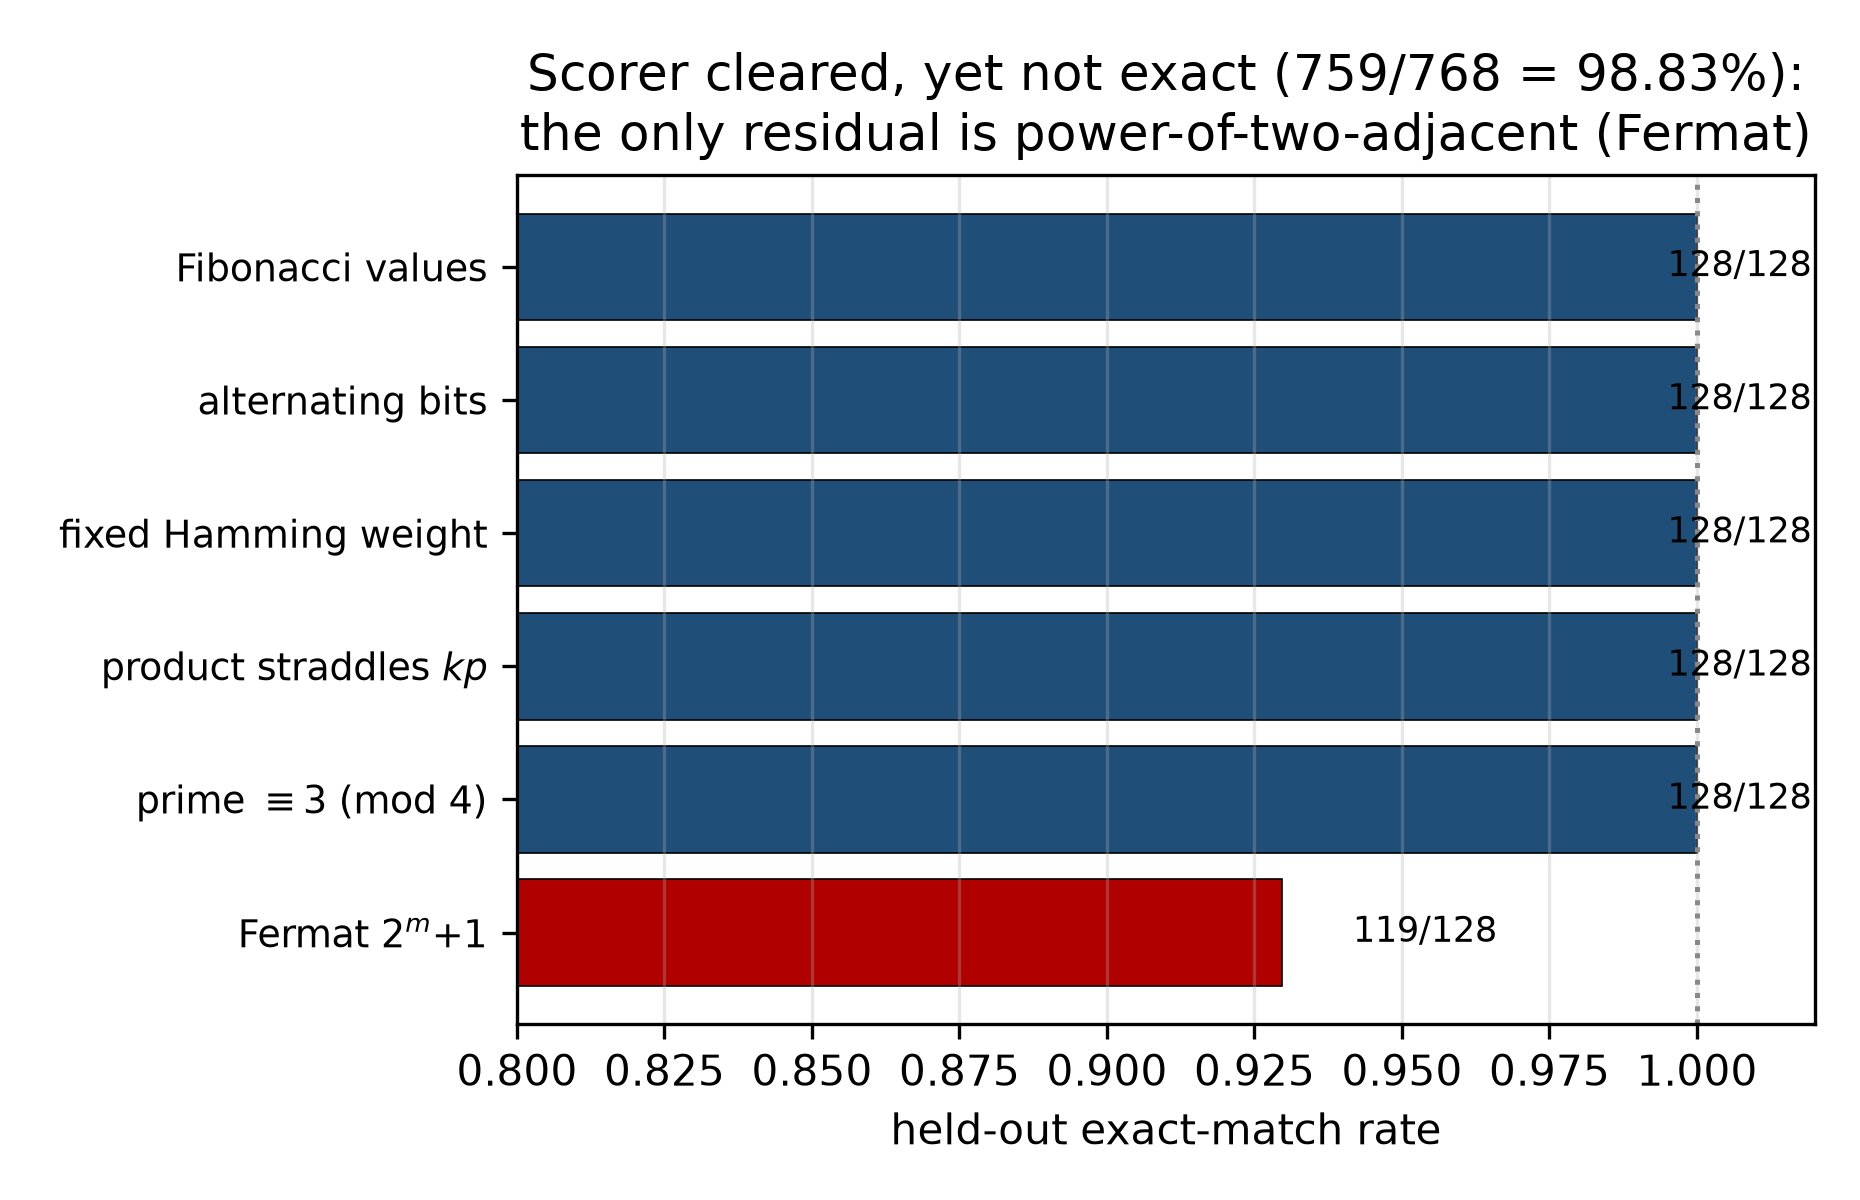
\includegraphics[width=0.82\linewidth]{figs/exactness_vs_depth.png}
 \caption{Submitted-v8 first-contact exact-match by operand family. The official scorer passes at
 $1.00$, yet the structured battery is not exact: five families are perfect and the
 only residual is the power-of-two-adjacent Fermat family ($119/128$), for an
 overall $759/768 = 98.83\%$.}
 \label{fig:exactness}
\end{figure}

% ============================================================
% LEAN
% ============================================================
\section{Machine-Checked Exactness of the Integer Algorithm}
\label{sec:lean}

A Lean~4 development addresses exactness at the level of the algorithm the loop
imitates, separately from the network. It does not mention the trained network, and
the gap between the two is stated explicitly.

\paragraph{The verified algorithm.}
Define the fold step
\[
 \mathrm{step}(s,d) \;=\; \bigl(2s + (\text{if } d \text{ then } x \text{ else } 0)\bigr) \bmod p ,
\]
run most-significant-bit-first over the bits of $b \bmod p$ with $x = a \bmod p$ and
initial state $s = 0$. The development machine-checks the following.

\begin{theorem}[double-and-add modular multiply]
For any prime $p$ and any operands $a, b$ of any bit length, folding
$\mathrm{step}$ MSB-first over the bits of $b \bmod p$ from $s = 0$ yields
$(a \cdot b) \bmod p$, and every intermediate state satisfies the canonical-residue
bound $s < p$.
\end{theorem}

The source contains neither \texttt{sorry} nor \texttt{admit}. Lean's axiom
report names only \texttt{propext} and \texttt{Quot.sound}. Both are standard axioms of Mathlib's
trusted base: \texttt{propext} is propositional extensionality (propositions with
the same truth value are equal), and \texttt{Quot.sound} is the soundness rule for
quotient types. They are used throughout Mathlib and add nothing task-specific, so
the result is complete modulo Lean's kernel and these two standard axioms. The
theorem certifies the integer double-and-add-mod-$p$ \emph{algorithm}.

\paragraph{A conditional exact-prefix bridge.}
The development additionally abstracts the implementation as an arbitrary
transition cell $C$. For one scan, \texttt{agreesFrom} recursively states that
$C$ equals $\mathrm{step}$ at the current exact state and along the exact
successor trajectory. Lean proves the following induction principle.

\begin{theorem}[exact-prefix trajectory certification]
If $C$ agrees with $\mathrm{step}$ at every exact-prefix state of a fixed bit
scan, then folding $C$ over that scan produces exactly the same final state as
folding $\mathrm{step}$. If this condition holds first for reduction and then
for the direct raw-bit scan using the exact residue, the two-pass cell rollout
equals $(a\cdot b)\bmod p$.
\end{theorem}

The single-scan theorem is axiom-free; the composed arithmetic corollary has
only the same \texttt{propext} and \texttt{Quot.sound} dependencies as the
modular arithmetic theorem above. This formalizes the logic used by the
exact-prefix trajectory runner: once every tested transition is exact, the
deterministic free-running path cannot diverge on that input.

\paragraph{The checkpoint-to-step bridge remains open.}
No weight tensor or GRU equation appears in the Lean development, and no theorem
proves that the submitted or repaired checkpoint satisfies
\texttt{agreesFrom} universally. Establishing that checkpoint-specific premise
beyond finite tested trajectories remains open. ``Provably exact'' is therefore
never claimed for the network. In particular, the theorem does not inspect or
certify the GRU weights; it says what follows \emph{if} the finite exact-prefix
premises hold for a fixed scan. The machine-checked conditional theorem and the
empirical exactness boundary of Section~\ref{sec:results} are complementary: the
first proves what a valid trajectory certificate entails; the second measures
where the learned cell actually supplies such certificates.

% ============================================================
% LIMITATIONS
% ============================================================
\section{Limitations}
\label{sec:limitations}

\paragraph{The submitted model is not exact.}
This is the central limitation and the reason the result is stated as a clean pass
of the benchmark distribution with cross-prime transfer, not as exact modular
multiplication. The power-of-two-adjacent residual (first-contact structured-battery $98.83\%$,
Section~\ref{sec:results:battery}) is real, and the recorded random-operand scorer
runs did not expose it.
A reader should not read $1.00$ on the scorer as exactness. Nor should the original
$759/768$ be read as a current sealed estimate, because later repair selection
used the same battery. The scorer's Tier-0
pure-multiplication diagnostic ($60/100$, Section~\ref{sec:results:tiers}) is a second,
sharper symptom of the same scoping: the cell realizes the modular product in its
training regime, not a general large-integer multiply. Counterexample-driven
training on the failing family, attempted here off-policy, did not cleanly close it,
it relocated the divergence to the multiply phase (Section~\ref{sec:results:battery}).
An immutable historical receipt records a later direct-two-pass/L2-SP candidate
as clearing the frozen-v3 exact-prefix $F_{11}$ induction gate, but the candidate
fails the broader frozen-v3 retention run at three
fixed-Hamming cases after $509/512$ exact attempted rows
(Section~\ref{sec:results:battery}); the other $1024$ rows were not run. The
four-arm causal ablation attributes the failures separately to a schedule effect,
a repaired-weight effect, and their interaction. This is a useful failed repair:
it rules out a tempting local-to-global inference and exposes a tested Pareto
wall, but it is not an impossibility result. The candidate is stopped, unsubmitted,
and unpromoted; submitted v8 remains the only qualified artifact.

\paragraph{The proof covers the algorithm, not the network.}
The machine-checked theorem (Section~\ref{sec:lean}) certifies the integer
double-and-add-mod-$p$ algorithm. It says nothing about the trained cell, and the
cell-to-step bridge is open.

\paragraph{Scale and hardware are not organizer-verified.}
The full-battery scores are the official open-source scorer, self-run on a single H100 rented via RunPod. Rob reports that the competition's automated submission evaluation returned the same
all-ten-tier result at $260$\,s. Its primary dashboard output is absent from this
workspace, so it is \texttt{ROB-CONFIRMED/UNARCHIVED}; it is not a human or organizer
verification, and the final ranked standing is not decided. The $163$--$174$\,s timing was measured on
the rented RunPod H100, and the organizers' hardware may differ. That local
headroom does not establish headroom or budget compliance on different hardware;
both remain unverified.

\paragraph{Compliance posture.}
The Horner schedule that drives the cell, the step count, the bit order, and
which argument supplies the control multiplier versus the data stream, is fixed
in advance rather than learned. Whether a fixed orchestration around a fully learned
arithmetic step falls on the permitted side of the
trained-parameters-versus-hand-coded-algorithm distinction is a question for the
organizers. As of this writing (August~2026), a clarification question is drafted
but has not been sent, and no ruling has been issued. The entry satisfies the
weight-perturbation anti-cheat condition: randomizing
the cell's weights collapses every tier to zero, the property the challenge names to
separate learned models from hand-coded circuits.

% ============================================================
% CONCLUSION
% ============================================================
\section{Conclusion}
\label{sec:conclusion}

Monolithic learners hit a wall on cross-prime modular multiplication: they fit
their training primes; monolithic learning of the task has had only limited success. A single
modulus-conditioned recurrent cell, reused across the reduce-reduce-multiply
schedule of a fixed bit-serial Horner loop, clears all ten tiers of the Modular
Arithmetic Challenge at exact-match $1.00$ on the official scorer, with
\texttt{overall\_accuracy} $1.00$ and \texttt{highest\_tier\_above\_90} of $10$,
reproduced across three seeds and within the time budget. One trained cell covers
every tier because dynamic state-width inference sizes the carried state to each
prime, a symbolically exact choice that was output-identical to full width on the
recorded finite comparison and, rather than kernel fusion, is what
brings a depth-bound run under budget; CUDA graphs were slower than the eager
baseline.

The mechanism is not new, and the model is not exact. XllentAI reported the same
learned modulus-conditioned Horner formulation and cross-prime transfer before
NeuralHorner's public release \citep{xllent2026horner}. The contribution here is
the compact single-checkpoint implementation with learned operand reductions,
together with a precise boundary: the random-operand scorer passes cleanly, while
the first-contact structured battery
isolated the only submitted-v8 residual to the power-of-two-adjacent Fermat family, $119/128$
where every other family was perfect. The single-step map and the integer algorithm
were respectively exact on the finite checked domain and machine-checked under
standard axioms, while the submitted-v8 learned chain breaks in this one specific
place.
The immutable historical receipt records the direct-two-pass/L2-SP candidate as
clearing a frozen-v3 vectorized exact-prefix induction gate on selected $F_{11}$
cases, yet its broader frozen-v3 retention run
fails after $509/512$ exact attempted rows at fixed-Hamming indexes $003$, $035$,
and $110$, with $1024$ rows left unrun by fail-closed stopping. The crossed
schedule/weight ablation classifies these as an interaction, a direct-schedule
failure, and a repaired-weight failure, respectively. The scientific result is
therefore a resolved negative one: the selected repair closes its target while
relocating error, and the cheaper route adds a separate vulnerable trajectory.
The candidate is stopped and was neither submitted nor promoted; v8 remains the
only qualified submission. A proof connecting either trained cell to the
machine-checked step also remains open: Lean proves a conditional exact-prefix
implication, not the checkpoint premise and not the weights themselves. Obtaining
a final leaderboard result is the remaining gate between the submitted-v8 scorer
evidence and a final competition claim.

\paragraph{Scaffold removal.}
We propose, but do not yet evaluate, a scaffold-removal program in which this entry is
the most-scaffolded point. The schedule is fixed here; the program would hand it back to
the network in stages, a learned controller over the same transition, a learned
latent state in place of explicit residue bits, then a recurrent bit processor, a looped
transformer, and a monolithic model, and measure where cross-prime transfer breaks,
the algorithmic-alignment trade-off \citep{velickovic2021nar, bohde2024markov}. Each
rung's transfer must be read against a settled base: the qualified submitted-v8
base still carries the characterized power-of-two-adjacent residual
(Section~\ref{sec:results:battery}), while the direct/L2-SP candidate failed
retention and is stopped. A higher rung's degradation would otherwise be confounded with the
base checkpoint's residual. We give the first rung a number. A small GRU controller, trained by imitation to drive
the loop schedule while the transition cell stays frozen, reproduces the Horner schedule
and extrapolates the per-step advance rule to twice the trained operand length at full
advance accuracy. But the per-step schedule error (about $1.6\%$ of continue steps)
compounds over the thousand-step rollout, so no full schedule is exactly correct at that
depth (zero whole-sequence-exact). Rung 1 thus measures the cost of removing the
hand-coded loop: a learned controller matches the schedule locally but not its exact
execution at depth, so the scaffold's contribution is the zero-error guarantee a learned
module did not exhibit in the recorded runs over thousands of steps. The higher rungs, learned latent state,
recurrent bit processor, looped transformer, monolithic, remain future work.

% ============================================================
% APPENDIX
% ============================================================
\appendix

\section{Methods and Reproducibility}
\label{app:repro}

\paragraph{Architecture.}
The learned cell is a bidirectional two-layer gated recurrent unit (GRU) of roughly
$471$K parameters, wrapped by the submission entry class
\texttt{model.BitSerialReducer}. The GRU was chosen over a plain RNN for gradient
stability over the long bit-serial rollout and over an LSTM for parameter economy
at matched width; bidirectionality lets each step condition on the full
carried-state bit vector. The architecture is not the contribution. The state is
carried as a bit vector, never as a wide integer, and the modulus enters only
through a conditioning input.

\paragraph{Training.}
The cell is trained from random initialization to predict the per-step transition
$s' = (2s + d\,x)\bmod p$ as a per-output-bit binary target, with no precomputed
tables. Training primes are generated by Miller--Rabin primality and stratified by
bit-length to span the tier widths; states $s$, multipliers $x$, and data bits $d$
are sampled with oversampling near the modular wrap boundary $s \approx p/2$, where
the conditional reduction is decided. Optimization is AdamW (peak learning rate
$1.5\times10^{-3}$, weight decay $0.01$) with a short warmup ($2.5\%$ of steps)
followed by cosine decay, batch size $256$ ($128$ at the widest state), for $40$K
steps ($20$K at the widest), selecting the checkpoint with the best held-out tier
score. Wider state widths are warm-started from a narrower trained cell, since the
transition is width-agnostic, which is what lets a single weight set cover the tier
ladder. A final on-policy DAgger pass \citep{DAgger2011} relabels the states the
cell actually visits during free-running reduce/reduce/multiply rollouts (powers of
two, sparse, all-ones, near-multiple, and multiply-control families) with the exact
transition, mixed with the sampler and refreshed every few thousand steps, to close
the long-chain drift that teacher-forced training leaves. Evaluation primes are
disjoint from training (a separate generator seed). The structured battery
families of Section~\ref{sec:results:battery} were not used to train submitted v8,
but later repair studies selected against them.

\paragraph{Inference.}
At evaluation the per-step state width is set to $\lceil \log_2 p \rceil$ for the
prime at hand (Section~\ref{sec:method:dynl}), with bit extraction in $32$-bit
limbs so that a modulus $p \ge 2^{63}$ never overflows an integer tensor. The loop
schedule, step count, and bit order are fixed by hand and identical across primes;
only the cell weights are learned.

\paragraph{Evaluation.}
{\sloppy
Scoring uses the challenge's official open-source scorer, run on a single H100 rented via
RunPod, distinct from the separate weight-perturbation anti-cheat battery below. The
official scorer's per-tier exact-match is reported over three independent seeds
(\texttt{a1a1a1a1}, \texttt{b2b2b2b2}, \texttt{c3c3c3c3}).
Each scored tier is $100/100$ in every run.
\texttt{overall\_accuracy} is $1.00$ and \texttt{highest\_tier\_above\_90} is $10$,
in every seed. A full run completes in $163$--$174$ seconds, about $125$ seconds
under the $300$-second budget, and the determinism re-run is identical.
\par}

The weight-perturbation anti-cheat battery is a separate, smaller check: $64$ cases per
tier per seed. Pooling the three seeds gives $192/192$ per tier, a $95\%$
Clopper--Pearson interval of $[0.981, 1.000]$. The provenance variant of this check
(Section~\ref{sec:method:output}) replaces the trained weights with random values of
matched shape and shows that every tier collapses from $64/64$ to $0/64$.

\paragraph{Precision and speed measurements.}
The $\mathrm{bf16}$ decision check (Section~\ref{sec:results:bf16}) found no
answer flips against $\mathrm{fp32}$ on this battery; its minimum decision margin
was $\min|\text{logit}| = 3.017$. This is a
\texttt{LOCAL-RESULT/UNARCHIVED} observation because the script is present but
its primary output log is not. The speed comparison
(Section~\ref{sec:method:speed}) records an eager baseline of $383$ seconds, a CUDA
graph variant at $402$ seconds, and the dynamic-state-width run at $163$--$174$
seconds.

\paragraph{Frozen structured battery.}
The structured battery (Section~\ref{sec:results:battery}) uses six families at
$128$ cases each, $768$ total, and the submitted v8 checkpoint scores $759/768$
($98.83\%$), with all nine failures in the power-of-two-adjacent Fermat family.
The families were disjoint from the original v8 training data and were first
scored after that checkpoint was frozen. Subsequent repair attempts were selected
against them, so the count is first-contact evidence for v8 and development
evidence thereafter, not a current sealed generalization estimate.
Generation, $N=128$ per family at the tier operand width $W$ with a held-out prime:
Fibonacci operands are drawn from the Fibonacci sequence; Fermat operands are
$2^{2^k}+1$ for $k$ with $2^{2^k}+1 < 2^{W}$, paired with random multipliers;
alternating-bit operands use the $\texttt{0x55\ldots}$/$\texttt{0xAA\ldots}$ patterns;
fixed-Hamming-weight operands carry exactly $W/2$ set bits. The generator's
legacy ``product straddles $kp$'' family samples a target $kp+\varepsilon$ but sets
$b=\lfloor(kp+\varepsilon)/a\rfloor$; the floor remainder is not controlled, so
the resulting products are quotient-correlated rather than reduction-boundary
cases. In the frozen $N=128$ set, $0/128$ products lie within distance $3$ of a
multiple of $p$ and nearest-boundary distances have 2040--2047 bits (median
2046). The cases and legacy key are preserved for receipt continuity, but no
boundary-stress claim is made. Finally,
the $p\equiv 3\pmod 4$ family fixes such a prime with random operands.

\paragraph{Reproducibility receipts.}
The checkpoint has $\sim$471K parameters and entry class
\texttt{BitSerial\allowbreak Reducer} in \texttt{model.py}. Its \texttt{weights.pt} MD5 prefix is
\texttt{8fc8ace7d745}. The scorer is the official \texttt{modchallenge}; the
environment is PyTorch~2.4 on a single NVIDIA H100 rented via RunPod. Seeds
\texttt{a1a1a1a1}, \texttt{b2b2b2b2}, \texttt{c3c3c3c3} gave per-run wall-clocks
$170$, $163$, $174$\,s, with an identical determinism re-run. The full artifact
digests are preserved in the repository receipts.

Provenance: weight-randomization collapse ($0/64$ every tier); the static
forward-path audit (no modular reduction, 3-arg \texttt{pow}, big-integer library,
lookup table, or comparison against $p$); and the bf16-vs-fp32 check ($0$ flips,
$\min|\text{logit}|
= 3.0$). The Lean development builds under Lean~4.31.0, is
\texttt{sorry}/\texttt{admit}-free, and reports axioms \texttt{propext},
\texttt{Quot.sound}. Commands:
\begin{verbatim}
modchallenge evaluate <submission> --total 1100
python scripts/verify_no_shortcut.py \
  <submission> --randomize
python scripts/held_out_battery.py <submission> --n 128
python scripts/audit_forward_path.py <submission>/model.py
cd lean && lake build
\end{verbatim}

\paragraph{Anticipated objections.}
\emph{The loop is hand-coded.} Correct, and stated as such (Table~\ref{tab:learned-vs-fixed}):
we study a learned transition inside a fixed scaffold; randomizing the cell collapses
every tier to zero, so the learned weights, not the schedule, carry the answer.
\emph{The model is not exact.} Correct; the residual is characterized to the
power-of-two-adjacent Fermat family and concentrates at $F_{11}=2^{2048}+1$ for
submitted v8. The immutable historical receipt records a direct/L2-SP candidate
passing the frozen-v3 exact-prefix induction gate on selected $F_{11}$ cases, but
the candidate then fails retention at three fixed-Hamming
cases; it is stopped and was never qualified, promoted, or submitted.
\emph{Hidden symbolic arithmetic.} The static forward-path audit and the
weight-randomization collapse are the receipts against it.
\emph{Dynamic-$L$ changes the computation.} It is exact for the symbolic recurrence
and output-identical to full-width inference on the recorded $6/6$ comparison.
\emph{This is not a new architecture or formulation.} Correct; learned
modulus-conditioned Horner transfer is prior art \citep{xllent2026horner}. The
contribution is the compact single-checkpoint learned-reduction implementation,
the measured failure boundary, and the verification stack.

% ============================================================
% ============================================================
\section*{Acknowledgments}
This work was developed by the author with Claude Opus 4.8 (Anthropic) in a
human-in-the-loop process. Receipt-backed quantitative claims were checked against
the stated artifacts and evaluation surfaces. The playground scores and automated
submission timing are labeled as Rob-confirmed but unarchived and are not
presented as independently verified. The bf16 comparison is separately labeled
as a local but unarchived result; its script is present but its primary output is
not. Available receipts are indexed in the repository.

% ============================================================
% BIBLIOGRAPHY
% ============================================================
\begin{thebibliography}{9}

\bibitem[Fan et al.(2024)]{fan2024looped}
Ying Fan, Yilun Du, Kannan Ramchandran, and Kangwook Lee.
\newblock Looped transformers for length generalization.
\newblock arXiv preprint arXiv:2409.15647, 2024.

\bibitem[Kaiser and Sutskever(2016)]{kaiser2016neural}
\L{}ukasz Kaiser and Ilya Sutskever.
\newblock Neural {GPU}s learn algorithms.
\newblock In \emph{International Conference on Learning Representations (ICLR)}, 2016.
 arXiv:1511.08228.

\bibitem[Lauter et al.(2024)]{lauter2024modular}
Kristin Lauter, Cathy Yuanchen Li, Krystal Maughan, Rachel Newton, and Megha Srivastava.
\newblock Machine learning for modular multiplication.
\newblock arXiv preprint arXiv:2402.19254, 2024.

\bibitem[XllentAI(2026)]{xllent2026horner}
XllentAI.
\newblock Horner-RNN: learned modular multiplication.
\newblock Hugging Face model repository, 2026. Historical formulation revision
\href{https://huggingface.co/XllentAI/modular_arithmetic/tree/3d2c226c2382140b890026bdfdd59485daa192ba}{3d2c226};
current snapshot as of August~1, 2026:
\href{https://huggingface.co/XllentAI/modular_arithmetic/tree/f704813dc64d7c04cc9ba7dbf9a3a281c431628d}{f704813}.

\bibitem[Lindner et al.(2023)]{lindner2023tracr}
David Lindner, J\'anos Kram\'ar, Sebastian Farquhar, Matthew Rahtz, Thomas McGrath,
 and Vladimir Mikulik.
\newblock Tracr: Compiled transformers as a laboratory for interpretability.
\newblock In \emph{Advances in Neural Information Processing Systems (NeurIPS)}, 2023.
 arXiv:2301.05062.

\bibitem[Price et al.(2016)]{price2016neural}
Eric Price, Wojciech Zaremba, and Ilya Sutskever.
\newblock Extensions and limitations of the {N}eural {GPU}.
\newblock arXiv preprint arXiv:1611.00736, 2016.

\bibitem[Weiss et al.(2018)]{weiss2018automata}
Gail Weiss, Yoav Goldberg, and Eran Yahav.
\newblock Extracting automata from recurrent neural networks using queries and
 counterexamples.
\newblock In \emph{International Conference on Machine Learning (ICML)}, 2018.
 arXiv:1711.09576.

\bibitem[Weiss et al.(2021)]{weiss2021rasp}
Gail Weiss, Yoav Goldberg, and Eran Yahav.
\newblock Thinking like transformers.
\newblock In \emph{International Conference on Machine Learning (ICML)}, 2021.
 arXiv:2106.06981.

\bibitem[Ross et al.(2011)]{DAgger2011} S.~Ross, G.~Gordon, and J.~A. Bagnell. A reduction of imitation learning and structured prediction to no-regret online learning. \emph{AISTATS}, 2011.

\bibitem[Velickovic and Blundell(2021)]{velickovic2021nar} Petar Veli\v{c}kovi\'c and Charles Blundell. Neural algorithmic reasoning. \emph{Patterns}, 2(7), 2021. arXiv:2105.02761.

\bibitem[Zhou et al.(2024)]{zhou2023rasp} Hattie Zhou, Arwen Bradley, Etai Littwin, Noam Razin, Omid Saremi, Josh Susskind, Samy Bengio, and Preetum Nakkiran. What algorithms can transformers learn? A study in length generalization. \emph{ICLR}, 2024. arXiv:2310.16028.

\bibitem[McCracken et al.(2025)]{mccracken2025modadd} Gavin McCracken, Gabriela Moisescu-Pareja, Vincent Letourneau, Doina Precup, and Jonathan Love. Uncovering a universal abstract algorithm for modular addition in neural networks. arXiv preprint arXiv:2505.18266, 2025.

\bibitem[Wenger et al.(2022)]{salsa2022} Emily Wenger, Mingjie Chen, Fran\c{c}ois Charton, and Kristin Lauter. SALSA: Attacking lattice cryptography with transformers. \emph{NeurIPS}, 2022. arXiv:2207.04785.

\bibitem[Wenger et al.(2024)]{salsafresca2024} Emily Wenger, Eshika Saxena, Mohamed Malhou, Ellie Thieu, and Kristin Lauter. Salsa Fresca: Angular embeddings and pre-training for ML attacks on learning with errors. arXiv preprint arXiv:2402.01082, 2024.

\bibitem[Reed and de Freitas(2016)]{reed2016npi} Scott Reed and Nando de Freitas. Neural programmer-interpreters. \emph{ICLR}, 2016. arXiv:1511.06279.

\bibitem[Bohde et al.(2024)]{bohde2024markov} Montgomery Bohde, Meng Liu, Alexandra Saxton, and Shuiwang Ji. On the Markov property of neural algorithmic reasoning: analyses and methods. \emph{ICLR}, 2024. arXiv:2403.04929.

\bibitem[Saxena et al.(2024)]{saxena2024modarith} Eshika Saxena, Alberto Alfarano, Fran\c{c}ois Charton, Zeyuan Allen-Zhu, Emily Wenger, and Kristin Lauter. Making hard problems easier with custom data distributions and loss regularization: a case study in modular arithmetic. arXiv preprint arXiv:2410.03569, 2024.

\bibitem[Power et al.(2022)]{power2022grokking} Alethea Power, Yuri Burda, Harri Edwards, Igor Babuschkin, and Vedant Misra. Grokking: generalization beyond overfitting on small algorithmic datasets. arXiv preprint arXiv:2201.02177, 2022.

\bibitem[Nanda et al.(2023)]{nanda2023progress} Neel Nanda, Lawrence Chan, Tom Lieberum, Jess Smith, and Jacob Steinhardt. Progress measures for grokking via mechanistic interpretability. \emph{ICLR}, 2023. arXiv:2301.05217.

\bibitem[Gromov(2023)]{gromov2023grokking} Andrey Gromov. Grokking modular arithmetic. arXiv preprint arXiv:2301.02679, 2023.

\end{thebibliography}

\end{document}
